\chapter{KIỂM TRA, TINH CHỈNH VÀ TIẾN HÀNH SẢN XUẤT}
    \section{KIỂM TRA VÀ TINH CHỈNH}
    \hspace{0.5cm} Sau khi hoàn thiện thiết kế và mô phỏng, bước tiếp theo là kiểm tra và tinh chỉnh hệ thống để đảm bảo hoạt động ổn định và hiệu quả. Quá trình này bao gồm:
    \begin{itemize}
        \item \textbf{Kiểm tra phần cứng}: Đảm bảo tất cả các thành phần cơ khí và điện tử được lắp ráp chính xác, không có lỗi kết nối hoặc hỏng hóc.
        \item \textbf{Kiểm tra phần mềm}: Chạy thử các thuật toán điều khiển và mô phỏng trong môi trường thực tế để phát hiện và sửa lỗi.
        \item \textbf{Tinh chỉnh tham số}: Điều chỉnh các tham số điều khiển như tốc độ động cơ, độ nhạy cảm biến, và các giá trị trong thuật toán để đạt được hiệu suất tối ưu.
    \end{itemize}
    \section{TIẾN HÀNH SẢN XUẤT}
    \hspace{0.5cm} Sau khi đã kiểm tra và tinh chỉnh thành công, tiến hành sản xuất robot theo thiết kế đã được phê duyệt. Quá trình sản xuất bao gồm:
        \subsection{Kết quả thiết kế cơ khí}
            \hspace{0.5cm} Thiết kế cơ khí của robot đã được hoàn thiện với các chi tiết được tối ưu hóa cho việc in 3D bằng vật liệu PLA
            \begin{figure}[H]
                \centering
                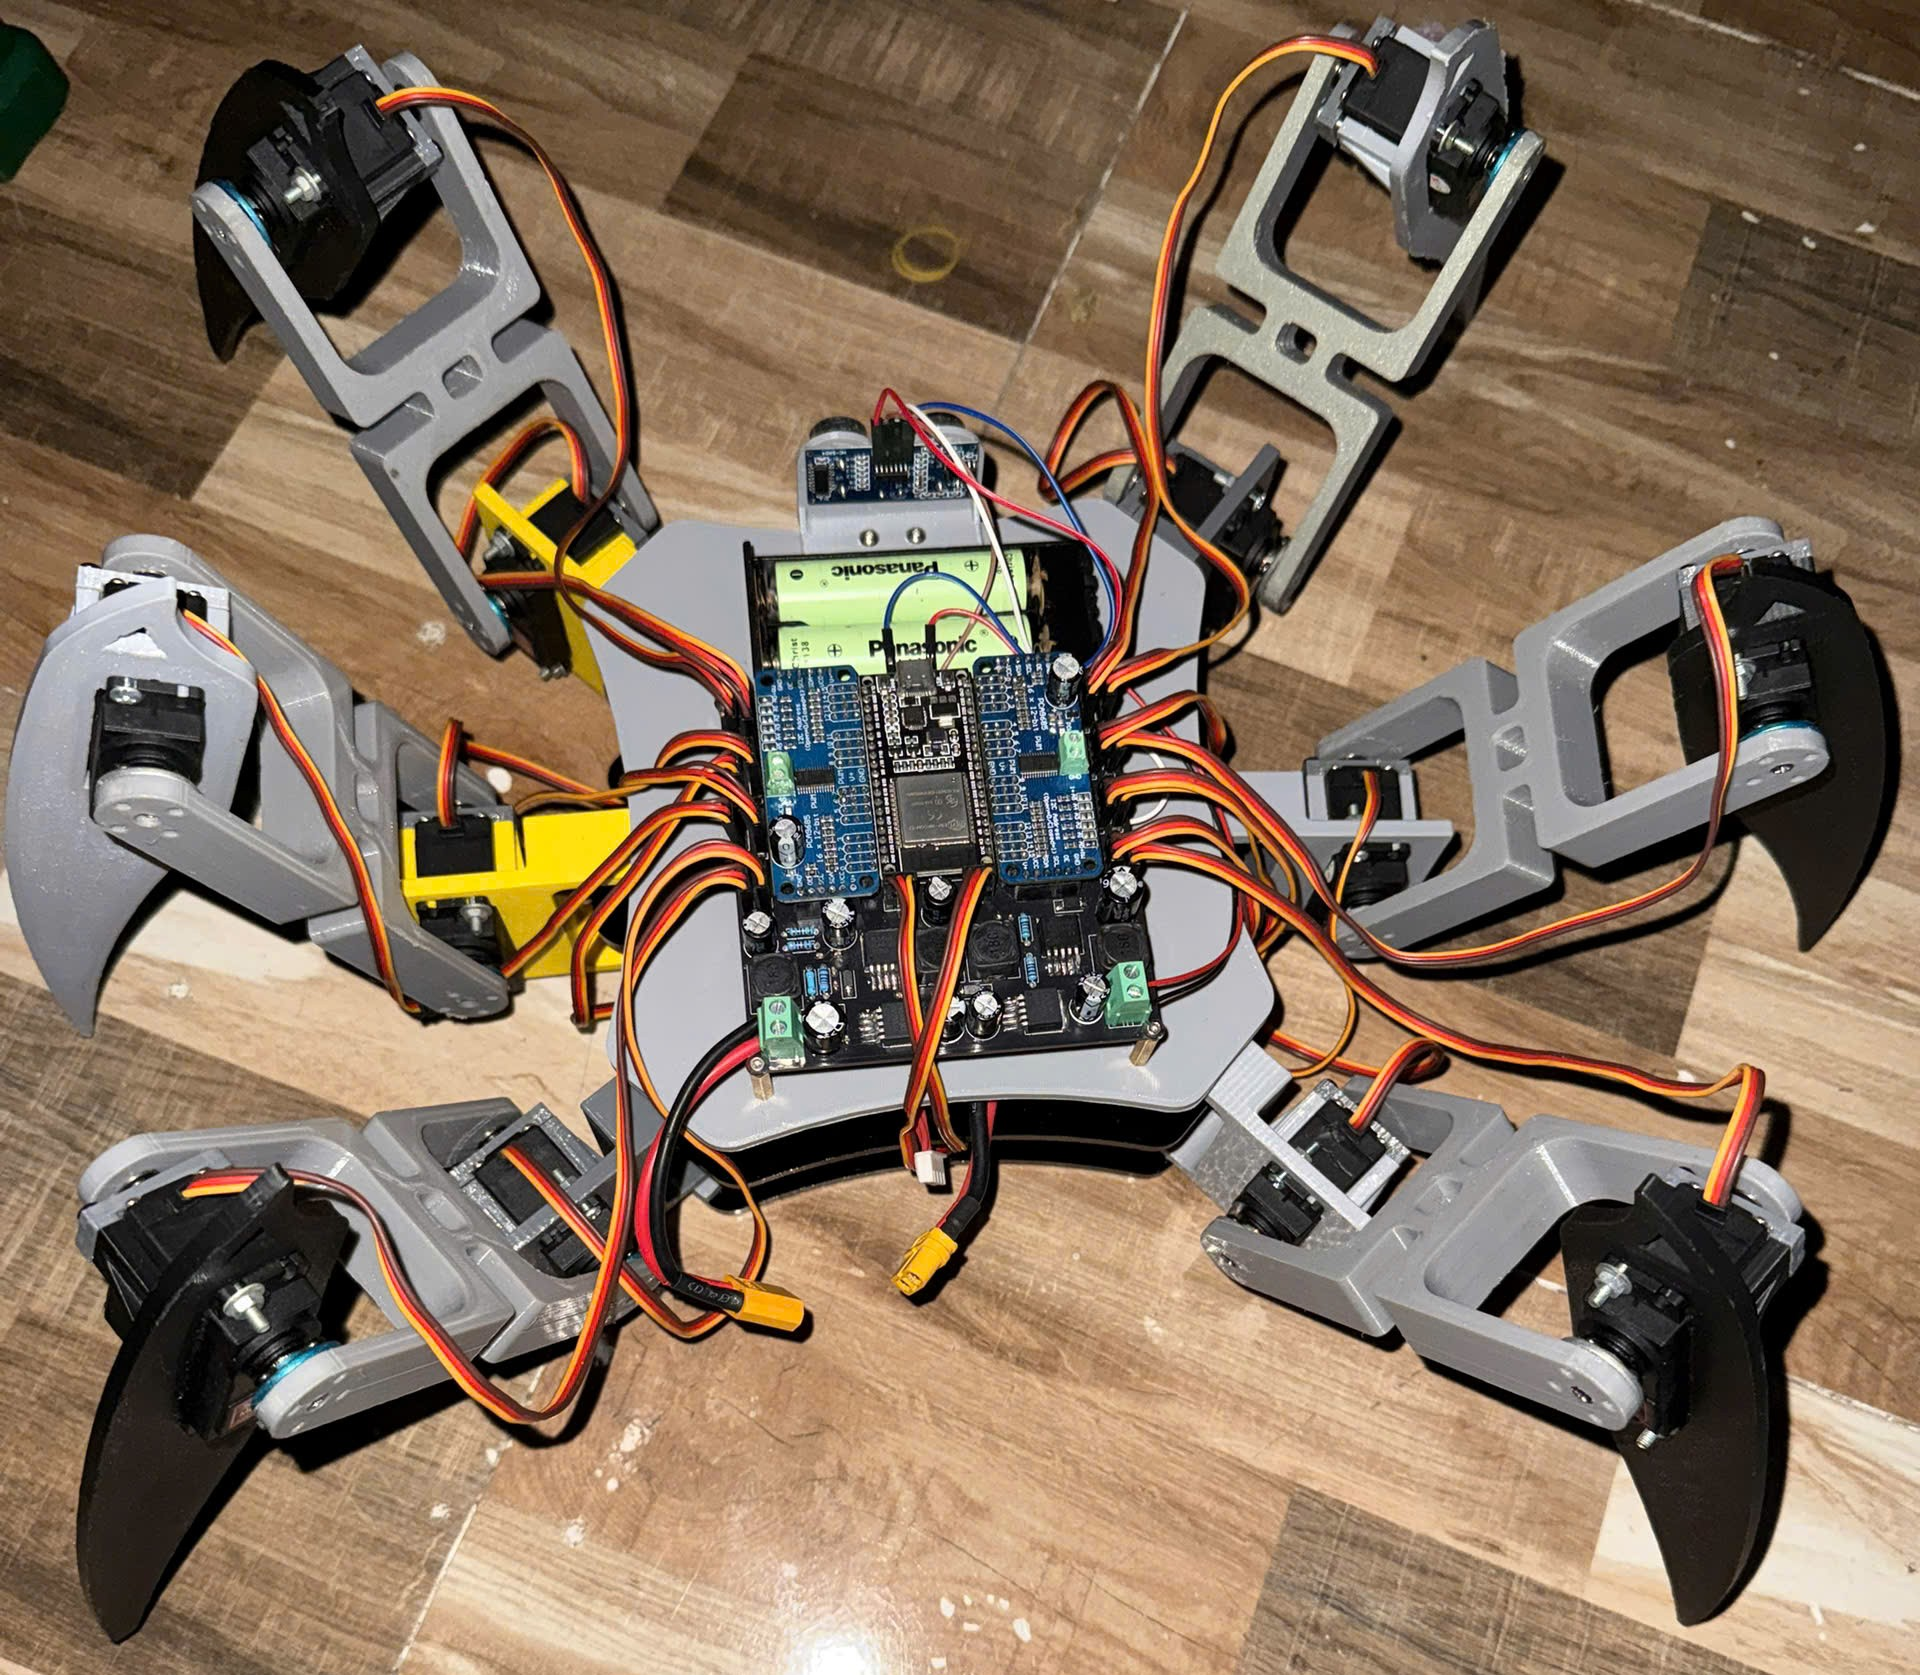
\includegraphics[width=0.75\textwidth]{pictures/robot.png}
                \caption{Robot sau khi lắp ráp}
            \end{figure}
            Các chi tiết như thân robot, chân, và khớp đã được thiết kế với độ dày và cấu trúc phù hợp để đảm bảo độ bền và khả năng chịu lực trong quá trình hoạt động.
        \subsection{Kết quả thiết kế điện}
            \hspace*{0.5cm} Mạch PCB đã được thiết kế và lắp ráp thành công với các linh kiện điện tử cần thiết để điều khiển robot. Mạch đã được kiểm tra và hoạt động ổn định, đảm bảo khả năng giao tiếp giữa các cảm biến, động cơ và bộ điều khiển trung tâm.
            \begin{figure}[H]
                \centering
                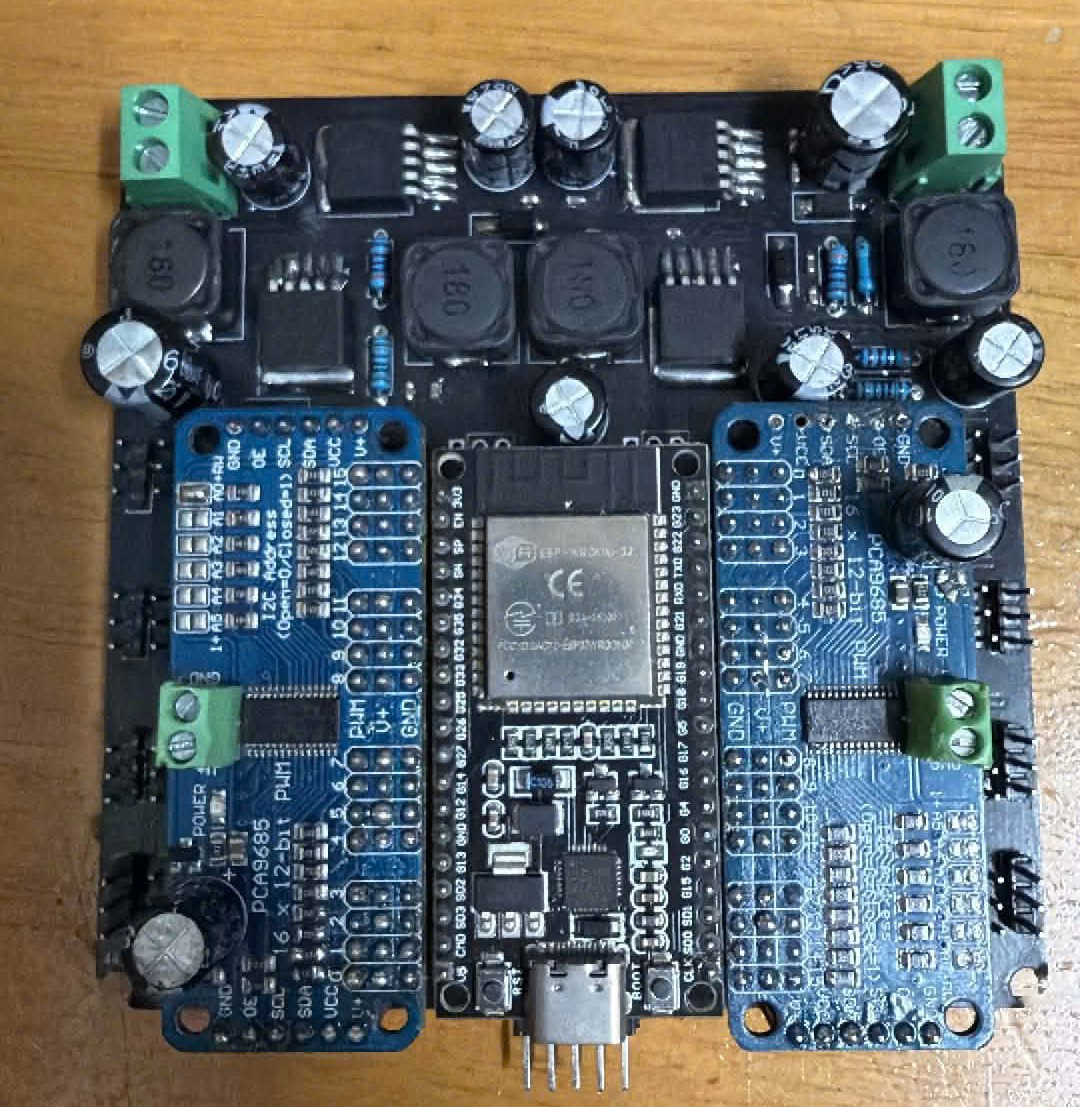
\includegraphics[width=0.75\textwidth]{pictures/pcb_assembled.png}
                \caption{Mạch PCB của robot sau khi hàn các linh kiện}
            \end{figure}
        \subsection{Kết quả thiết kế phần mềm}
            \hspace*{0.5cm} Giao diện web đã được phát triển và kiểm tra thành công, cho phép người dùng điều khiển robot một cách trực quan và hiệu quả. Các chức năng như di chuyển, thay đổi các tham số, theo dõi chuyển động, và thực hiện các hành động đặc biệt đã được tích hợp và hoạt động ổn định.
            \begin{figure}[H]
                \centering
                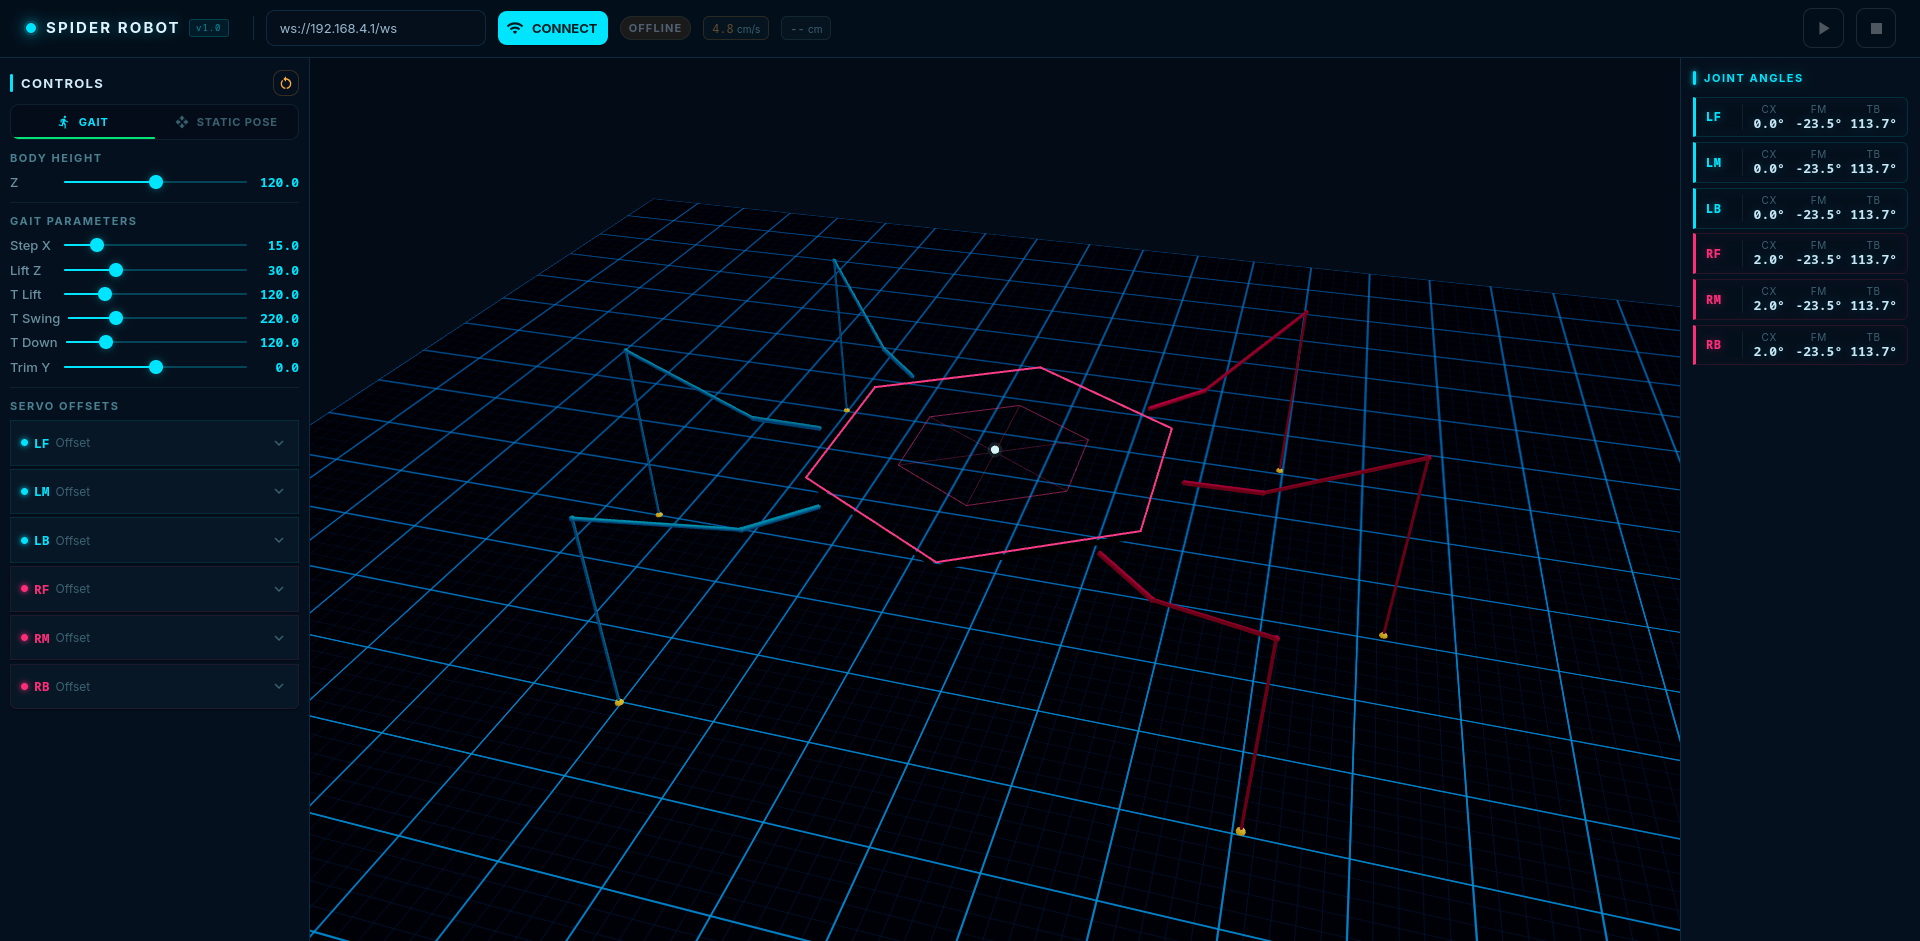
\includegraphics[width=0.75\textwidth]{pictures/software_system.png}
                \caption{Giao diện kiểm tra phần mềm điều khiển robot}
            \end{figure}
            \begin{figure}[H]
                \centering
                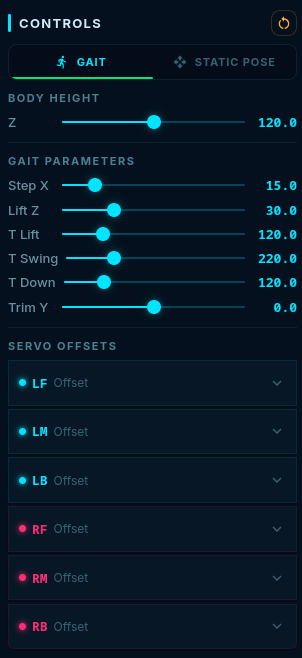
\includegraphics[width=0.3\textwidth]{pictures/gait_mode.png}
                \caption{Giao diện điều khiển robot chế độ GAIT}
            \end{figure}
            \begin{figure}[H]
                \centering
                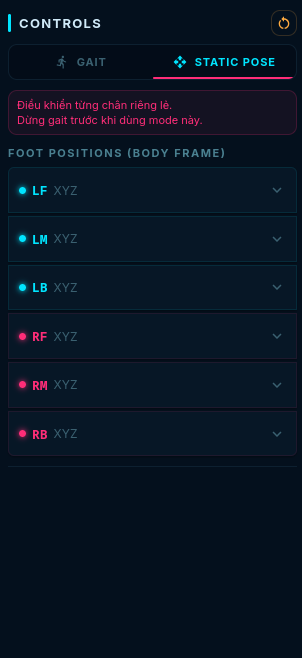
\includegraphics[width=0.3\textwidth]{pictures/static_mode.png}
                \caption{Giao diện điều khiển robot chế độ STATiC}
            \end{figure}
            